% Camera to LaTeX: Set-up Guide (Revision 2 of docs/instructions.pdf)
% Build:  pdflatex setup_guide.tex   (run it twice for the table of contents)
\documentclass[11pt,letterpaper]{article}
\usepackage{guidestyle}
\renewcommand{\guidetitle}{Camera to \LaTeX{}: Set-up Guide}
\hypersetup{pdftitle={Camera to LaTeX: Set-up Guide},pdfauthor={EE 105 Team 8}}

\begin{document}
\thispagestyle{plain}
\guidefront{Camera to \LaTeX{}: Set-up Guide}%
  {Installation and Quick Start on Windows, from an Empty Computer to a Working Pipeline}%
  {EE\,105, Fall 2026 \textperiodcentered{} Team 8 \textperiodcentered{} Revision 2 of the project instructions}%
  {November 24, 2026}

\begin{quote}
\small
\textbf{Abstract.} This guide takes a team member whose Windows laptop holds none of the
project's software to the point at which the complete Camera-to-\LaTeX{} pipeline runs on that
laptop without the camera board. By the end, the reader has a GitHub account with access to the
team's repository, a local copy of the project, a working Python environment, a passing test
suite, a trained symbol classifier, and a typeset PDF produced from a simulated camera photograph
of a printed equation. Every action is written as a numbered step that states the exact command,
the result to expect, and the remedy when the result differs. No prior knowledge of Git, Python,
the command line or \LaTeX{} is assumed. Work with the camera board itself is the subject of the
companion document, \emph{Procedures for the Remaining Tasks}.
\end{quote}

\begin{table}[H]
\centering
\begin{tabular}{C{1.5cm}L{5.2cm}C{1.9cm}C{2.0cm}}
\toprule
\hd{Section} & \multicolumn{1}{c}{\hd{What you do}} & \hd{Time} & \hd{Download} \\
\midrule
\ref{sec:prelim} & Check that the laptop is suitable & 5 min & none \\
\ref{sec:github} & Create a GitHub account and obtain access to the repository & 15 min & none \\
\ref{sec:powershell} & Learn to open and use Windows PowerShell & 10 min & none \\
\ref{sec:tools} & Install Git, Python, MiKTeX and Poppler & 40 min & 0.5 GB \\
\ref{sec:clone} & Download the project and introduce yourself to Git & 10 min & 2 MB \\
\ref{sec:python} & Build the Python environment & 30 min & 0.6 GB \\
\ref{sec:quick} & Run the quick start: tests, data, training, evaluation, PDF & 90 min & 0.1 GB \\
\bottomrule
\end{tabular}
\caption{The route through this guide. Times are typical for a home internet connection; about
60 min of the quick start is unattended (the laptop trains the classifier by itself). The
installed software occupies about 4 GB of disk space.}
\label{tab:route}
\end{table}

\tableofcontents
\clearpage
\section{Introduction}
\label{sec:intro}

\subsection{What the project does}

The project reads one printed line of text or mathematics with a small camera and reproduces it
as a typeset document. The camera is the OV7675 module on the USC EE\,105 board, which carries an
Arduino Nano 33 BLE Sense Lite. The board has too little memory to do more than take the
photograph (256\,KB of RAM against 76{,}800 bytes for a single $320 \times 240$ grayscale frame),
so it sends each frame to a laptop over the USB cable, and the laptop does the rest. The sequence
of processing steps on the laptop is called the \term{pipeline}; Figure~\ref{fig:pipeline} shows
it.

\begin{figure}[H]
\centering
\begin{tikzpicture}[node distance=7mm, every node/.style={font=\small},
  box/.style={draw, rounded corners=2pt, align=center, minimum height=12mm, inner sep=2.5pt, text width=23mm},
  >={Stealth[length=2mm]}]
\node[box, fill=black!6] (b) {Board\\\scriptsize camera, sketch};
\node[box, right=of b] (c) {Capture\\\scriptsize 320\,$\times$\,240 gray};
\node[box, right=of c] (s) {Segment\\\scriptsize one box per symbol};
\node[box, right=of s] (k) {Classify\\\scriptsize CNN, 159 classes};
\node[box, below=8mm of k] (l) {Layout\\\scriptsize scripts, fractions};
\node[box, left=of l] (t) {\LaTeX{} line\\\scriptsize compile check};
\node[box, left=of t] (p) {PDF\\\scriptsize pdflatex};
\draw[->] (b) -- node[above, font=\tiny, inner sep=1.5pt]{USB} (c);
\draw[->] (c) -- (s);
\draw[->] (s) -- (k);
\draw[->] (k) -- (l);
\draw[->] (l) -- (t);
\draw[->] (t) -- (p);
\end{tikzpicture}
\caption{The pipeline. Only the shaded box runs on the board. This guide installs and tests every
unshaded box, using stored photographs in place of the board.}
\label{fig:pipeline}
\end{figure}

The stages are as follows. \emph{Capture} receives a frame from the board. \emph{Segment} finds
the ink in the frame and draws one box around each printed symbol. \emph{Classify} passes each
boxed symbol to a convolutional neural network (CNN), which names it as one of 159 classes
covering the visible ASCII characters and the common mathematical symbols. \emph{Layout} decides
how the symbols relate to one another (which are superscripts, subscripts, numerators or
denominators) and writes the corresponding \LaTeX{} text. Finally the program \cmd{pdflatex}
turns that text into a PDF.

\subsection{What you will have at the end}

A reader who completes every checkpoint of this guide has:
\begin{itemize}
\item a GitHub account that can read from, and write to, the team's repository;
\item the tools Git, Python 3.12, MiKTeX and Poppler installed and verified;
\item the project in the folder \file{C:\bs ee105\bs camera-to-latex}, with its own Python
  environment;
\item a passing run of the project's automatic tests;
\item a trained classifier and a measured accuracy on 80 simulated camera photographs;
\item a PDF, opened on screen, that the pipeline produced from a photograph of an equation.
\end{itemize}
At that point the laptop is ready for the tasks that use the board.

\subsection{Assumptions and scope}

The guide makes four assumptions and no others.
\begin{enumerate}
\item The laptop runs 64-bit Windows 10 or Windows 11 on an Intel or AMD processor.
  Section~\ref{sec:prelim} shows how to check this.
\item You can install software on it, which means that you know the password Windows asks for
  when a program requests permission to make changes.
\item It has an internet connection and at least 10\,GB of free disk space.
\item None of the project's software is installed, and you have not used any of it before.
\end{enumerate}
A team member whose laptop runs macOS or Linux should speak to the project lead before starting:
the project works on those systems (the short instructions are in the file \file{README.md}), but
the installation steps in Sections~\ref{sec:powershell} to~\ref{sec:python} are written for
Windows only.

If part of the software is already installed, do not skip the corresponding step; carry out its
verification instead (each installation step ends with one). If the verification succeeds, move
on.

\begin{note}[Status of this revision]
The commands of the project itself (Sections~\ref{sec:python} and~\ref{sec:quick}) were run by
the project lead on a Windows laptop on 23 November 2026, and their outputs are quoted from that
run. The installation steps of Sections~\ref{sec:tools} and~\ref{sec:clone} follow the
publishers' instructions (listed in the Sources appendix) and the lead's experience, but this
revision has not yet been followed from its first step to its last on a second, empty laptop.
The first team member to do so is asked to report every point at which the screen differed from
the description, so that the guide can be corrected.
\end{note}

\subsection{How to read this guide}
\label{sec:conventions}

The guide is meant to be followed in order, one step at a time, with this document open beside
the windows in which you work. Steps are numbered within their section: Step~5.3 is the third
step of Section~5. Four kinds of box appear.

\begin{ps}
Get-Date
\end{ps}

A blue box holds \emph{exactly one command} for Windows PowerShell, the program introduced in
Section~\ref{sec:powershell}. Type the line exactly as printed, or copy it from this PDF and
paste it, and then press \key{Enter}. Upper and lower case, spaces, hyphens, quotation marks and
backslashes all matter. A command is always printed on a single line; if two blue boxes follow
each other, they are two commands, and the first must finish before the second is typed.

\begin{out}
Tuesday, November 24, 2026 9:41:07 AM
\end{out}

A gray box shows what appears on the screen after the command. Your screen will rarely match it
character for character (dates, version numbers and folder names differ); the text below each
gray box says which part matters.

\begin{iffail}
An amber box describes the most likely way in which a step goes wrong, and the remedy.
Section~\ref{sec:trouble} collects all of them, with the exact error messages, in one place.
\end{iffail}

\begin{note}
A green box gives background that is useful but not needed to carry out the step.
\end{note}

Three further conventions are used throughout.
\begin{itemize}
\item \textbf{Keys} are drawn like this: \key{Enter}, \key{Ctrl}+\key{C} (hold the first key and
  press the second).
\item \textbf{Things to click} are printed in bold sans-serif type, for example \ui{Sign up}, and
  a path through menus is written with arrows: \menu{Settings}\then\menu{System}\then\menu{About}.
\item \textbf{Placeholders}, which you must replace with your own information, are printed in
  capitals on a yellow background, for example \ph{YOUR-NAME}. There are only four in the whole
  guide. Nothing else in a command is ever to be replaced, and no command in this guide contains
  the characters \code|<| or \code|>| around a word.
\end{itemize}

Each step ends with a \ok~\textbf{Checkpoint}: an observable fact that tells you the step
succeeded. Do not go on to the next step until the checkpoint is true.

\subsection{When you are stuck}
\label{sec:help}

First read the amber box of the step, then the entry for your error message in
Section~\ref{sec:trouble}. If neither resolves the problem, send the project lead three things:
the step number, a screenshot of the whole PowerShell window (press
\key{Windows}+\key{Shift}+\key{S}, drag a rectangle over the window, and paste the picture into
a message with \key{Ctrl}+\key{V}), and one sentence saying what you expected. Do not retype an
error message by hand, and do not experiment with commands found elsewhere; an installation that
has been altered by trial and error is much harder to repair than one that stopped at a known
step.

\section{Check the laptop}
\label{sec:prelim}

These three checks take five minutes and prevent the most expensive kind of failure, an
installation that cannot work on the machine at all.

\step{Find the Windows version}
Hold the \key{Windows} key (the key with the four-pane logo, next to \key{Alt}) and press
\key{R}. A small window titled \ui{Run} opens. Type \code|winver| in its box and press
\key{Enter}. A window titled \ui{About Windows} appears; read its first lines and then close it
with \ui{OK}.
\checkpoint{The window says \emph{Windows 10} or \emph{Windows 11}. For Windows 10 the version
shown must be 1809 or later (for example 22H2).}

\step{Find the processor type}
Click the \ui{Start} button, type \code|about your pc| and press \key{Enter}. The Settings
window opens on a page headed \ui{About}. Under \ui{Device specifications}, find the line
\ui{System type}.
\checkpoint{The line reads \emph{64-bit operating system, x64-based processor}.}

\begin{iffail}[If the line says ``ARM-based processor'' or ``32-bit'']
Stop here and tell the project lead. The neural-network library used by the project
(TensorFlow) is published for x64 processors only. The rest of the software can still be
installed, and the project's simpler fallback classifier works without TensorFlow, but the lead
should decide how your laptop is used.
\end{iffail}

\step{Find the free disk space}
Hold \key{Windows} and press \key{E} to open File Explorer. In its left-hand list click
\ui{This PC}. Under \ui{Devices and drives}, read the text below the drive named
\ui{Local Disk (C:)} or \ui{Windows (C:)}.
\checkpoint{At least 10\,GB is free on drive C:.}

\step{Show file name extensions}
The guide refers to files by their full names, such as \file{config.py} or \file{T26.png}.
Windows hides the part after the dot unless told otherwise. In File Explorer on Windows~11,
click \menu{View}\then\menu{Show}\then\menu{File name extensions}; on Windows~10, click the
\menu{View} tab and tick the box \ui{File name extensions}.
\checkpoint{File names in File Explorer now end in a dot and a few letters, for example
\file{.pdf} or \file{.png}.}

\section{A GitHub account and access to the repository}
\label{sec:github}

\subsection{Background}

\term{Git} is a program that records the history of a folder of files: every saved state (a
\term{commit}) can be recalled, compared and shared. A folder managed by Git is called a
\term{repository}. \term{GitHub} is a website that stores repositories on the internet so that
several people can work on the same one. The team's repository is

\begin{center}
\repourl
\end{center}

and it belongs to the project lead, Andrew Shahvosian, whose GitHub user name is
\texttt{ashahvos}. To read the repository you may need an account that the lead has invited; to
contribute to it you certainly do. The whole section is done in a web browser (Edge, Chrome or
Firefox); nothing is installed yet.

\subsection{Create the account}

Skip to Step~\ref{st:sendname} if you already have a GitHub account and can sign in to it.

\step{Open the sign-up page}
Open the browser, click in the address bar at the top, type the following address and press
\key{Enter}.
\begin{center}\url{https://github.com/signup}\end{center}
\checkpoint{A page headed \emph{Sign up for GitHub} (or similar) asks for an email address.}

\step{Fill in the form}
The layout of the page changes from time to time, but it always asks for the same four items.
\begin{enumerate}
\item \textbf{Email.} Enter an address whose inbox you can open right now; your USC address is a
  good choice.
\item \textbf{Password.} GitHub accepts a password of at least 15 characters, or of at least 8
  characters that include a number and a lowercase letter. Do not reuse a password from another
  site, and store it in a password manager or write it down now.
\item \textbf{Username.} This name is public and appears on every contribution you make. Use
  letters, digits and single hyphens only. A recognizable form of your own name is best, for
  example the part of your USC address before the \code|@| sign.
\item \textbf{Country or region.} Select it from the list.
\end{enumerate}
Leave any box about product updates unticked unless you want the emails, then click the button
at the bottom of the form (\ui{Create account} or \ui{Continue}).

\step{Prove that you are a person and confirm the email address}
GitHub shows a short visual puzzle; solve it. It then sends a numeric code to the email address
you gave. Open your inbox in another browser tab, find the message from GitHub (check the spam
folder if it has not arrived after two minutes), and type the code into the sign-up page.
\checkpoint{The browser shows your GitHub home page, or a sign-in page that accepts your new
user name and password. Any questions about your interests can be skipped with the link
\ui{Skip personalization} (or \ui{Skip this for now}); the free plan is sufficient.}

\begin{note}[Two-factor authentication]
GitHub strongly recommends, and for people who contribute code may require, a second sign-in
factor such as an authenticator app on your phone. If GitHub asks you to set it up, follow its
instructions; the request is genuine, and it does not interfere with anything in this guide.
\end{note}

\subsection{Obtain access}

\step{Send your user name to the project lead}\label{st:sendname}
Send Andrew a message through the team's usual channel that contains your GitHub user name
exactly as you typed it, including any hyphens. Then wait for his reply; he carries out
Step~\ref{st:invite}.
\checkpoint{The lead has confirmed that the invitation was sent.}

\step{For the project lead only: invite the team member}\label{st:invite}
\begin{enumerate}
\item Sign in to GitHub and open the page of the repository,\\ \repourl.
\item Click the \ui{Settings} tab of the repository (the rightmost tab under the repository
  name; if it is hidden, open the \ui{\ldots} menu at the end of the row of tabs).
\item In the left-hand list, under \ui{Access}, click \ui{Collaborators}. GitHub may ask for
  your password again.
\item Click \ui{Add people}, type the team member's user name, select the matching account in
  the list, and click the green button that names the account and the repository.
\end{enumerate}
The same page shows whether the repository is \emph{Private} or \emph{Public}. A private
repository cannot be seen at all by an account that has not accepted an invitation.
\checkpoint{The team member's name is listed on the Collaborators page with the remark
\emph{Pending invite}.}

\step{Accept the invitation}
GitHub sends you an email which says that \texttt{ashahvos} has invited you to collaborate on
the repository \texttt{ashahvos/camera-to-latex}. Open it and click \ui{View invitation}, then
\ui{Accept invitation}.
If the email cannot be found, sign in to GitHub and open this address instead:
\begin{center}\url{https://github.com/ashahvos/camera-to-latex/invitations}\end{center}
An invitation expires after seven days; if yours has expired, ask the lead to send it again.
\checkpoint{The browser shows the repository page: a list of folders and files
(\file{firmware}, \file{model}, \file{pipeline}, \file{tools}, \ldots) and, below it, the text of
the file \file{README.md} under the heading \emph{Camera to LaTeX}.}

\subsection{A first look at the repository}

\step{Read a file in the browser}
Nothing needs to be installed to read the project. On the repository page, click the folder
\file{docs}, then a PDF file in it; GitHub displays the document, and the download button
(an arrow pointing into a tray, at the top right of the file view) saves a copy. Click the
repository name \ui{camera-to-latex} at the top of the page to return to the start. The same
method works for \file{sheets/sheets.pdf} and \file{test\_set/test\_lines.pdf}, the two documents
that will later be printed.
\checkpoint{You have opened one file of the repository and returned to its first page.}

Table~\ref{tab:repo} lists what the repository contains. The names will become familiar in the
quick start of Section~\ref{sec:quick}.

\begin{table}[H]
\centering
\begin{tabular}{L{3.5cm}L{8.1cm}}
\toprule
\multicolumn{1}{c}{\hd{Name}} & \multicolumn{1}{c}{\hd{Contents}} \\
\midrule
\file{README.md} & A one-page summary of the project and its commands \\
\file{config.py} & Every adjustable number of the pipeline, in one file \\
\file{symbols.csv} & The 159 classes (182 symbols) the classifier knows \\
\file{requirements.txt} & The Python packages the project needs \\
\file{firmware/capture/} & The program (``sketch'') that runs on the board \\
\file{pipeline/} & Capture, segmentation, classification, layout, PDF output and the application \\
\file{model/} & Generation of training images, training and evaluation of the classifier \\
\file{tools/} & Printable sheets, test lines, evaluation and review of results \\
\file{sheets/} & The printable sheets of symbols (\file{sheets.pdf}, 9 pages) \\
\file{test\_set/} & The 80 test lines (\file{lines.tsv}, \file{test\_lines.pdf}) and their photographs \\
\file{tests/} & Automatic tests of the code \\
\file{docs/} & This guide and its companion \\
\bottomrule
\end{tabular}
\caption{The contents of the repository.}
\label{tab:repo}
\end{table}

\section{Windows PowerShell}
\label{sec:powershell}

\subsection{Background}

Most of the project is operated by typing commands rather than by clicking. A program that
accepts typed commands is called a \term{terminal} or \term{command line}; the one that every
Windows computer already contains is \term{Windows PowerShell}. A command is one line of text.
When you press \key{Enter}, PowerShell carries the line out, prints whatever the command
reports, and then waits for the next line. Nothing in this guide requires PowerShell to be
started ``as administrator'', and you should not start it that way.

\subsection{Open a PowerShell window}

\step{Open PowerShell}\label{st:openps}
Click the \ui{Start} button (or press the \key{Windows} key), type \code|powershell|, and wait
for the search results. Click the result named \ui{Windows PowerShell} whose description is
\emph{App}. Do \emph{not} choose \emph{Windows PowerShell ISE}, \emph{Windows PowerShell (x86)}
or \emph{Command Prompt}; they behave differently.

A window with a dark background opens. On Windows~11 it is usually a window of the
\emph{Terminal} app with a tab labelled \emph{Windows PowerShell}; on Windows~10 it is a blue or
black window titled \emph{Windows PowerShell}. Both are the same program.

\begin{out}[What the new window shows]
Windows PowerShell
Copyright (C) Microsoft Corporation. All rights reserved.

PS C:\Users\ttrojan>
\end{out}

\checkpoint{The last line begins with \texttt{PS}, shows a folder name, and ends with
\texttt{>} followed by a blinking cursor. On your computer the folder is
\texttt{C:\bs Users\bs} followed by your own Windows user name.}

\subsection{Read the prompt}

The last line of the window is the \term{prompt} (Figure~\ref{fig:prompt}). It has three parts.
\texttt{PS} says that PowerShell is ready for a command. The path after it, here
\code|C:\Users\ttrojan|, is the \term{current folder}: commands that mention a file look for it
in this folder unless told otherwise. The sign \code|>| marks the place where your typing
appears. The prompt is printed by PowerShell; you never type it, and it is not part of any
command in this guide.

\begin{figure}[H]
\centering
\begin{tikzpicture}[font=\ttfamily\small, seg/.style={fill=black!88, text=white, inner xsep=0pt, inner ysep=7pt, outer sep=0pt, anchor=west},
  lab/.style={font=\rmfamily\footnotesize, align=center, text=black}]
\node[seg, inner xsep=0pt] (pad) at (0,0) {\hspace{7pt}};
\node[seg, text=green!70!white] (a) at (pad.east) {(.venv)\vphantom{Ag>}};
\node[seg] (b) at (a.east) {\ PS\ \vphantom{Ag>}};
\node[seg] (c) at (b.east) {C:\textbackslash ee105\textbackslash camera-to-latex>\vphantom{Ag}};
\node[seg] (d) at (c.east) {\ python -m pytest -q\hspace{7pt}\vphantom{Ag>}};
\draw[decorate, decoration={brace, mirror, amplitude=4pt}] ($(a.south west)+(0,-0.08)$) -- ($(a.south east)+(0,-0.08)$);
\draw[decorate, decoration={brace, mirror, amplitude=4pt}] ($(b.south west)+(0.12,-0.08)$) -- ($(b.south east)+(-0.12,-0.08)$);
\draw[decorate, decoration={brace, mirror, amplitude=4pt}] ($(c.south west)+(0,-0.08)$) -- ($(c.south east)+(0,-0.08)$);
\draw[decorate, decoration={brace, mirror, amplitude=4pt}] ($(d.south west)+(0.15,-0.08)$) -- ($(d.south east)+(-0.25,-0.08)$);
\node[lab, anchor=north] at ($(a.south)+(-0.35,-0.95)$) {active environment\\(Section~\ref{sec:python})};
\draw[black!50] ($(a.south)+(0,-0.3)$) -- ($(a.south)+(-0.35,-0.95)$);
\node[lab, anchor=north] at ($(b.south)+(0,-0.3)$) {ready};
\node[lab, anchor=north] at ($(c.south)+(0,-0.3)$) {current folder};
\node[lab, anchor=north] at ($(d.south)+(0,-0.3)$) {the command you typed};
\end{tikzpicture}
\caption{The parts of a PowerShell line as it will look later in this guide. Everything to the
left of the command is the prompt, which PowerShell prints by itself.}
\label{fig:prompt}
\end{figure}

\subsection{Type, paste and run commands}

\step{Run a first command}
Click once inside the window, type the following line, and press \key{Enter}.
\begin{ps}
Get-Location
\end{ps}
\begin{out}
Path
----
C:\Users\ttrojan

PS C:\Users\ttrojan>
\end{out}
\checkpoint{PowerShell printed the current folder and then a new prompt. The new prompt is the
sign that the command has finished; a command is still running for as long as no prompt has
appeared.}

\step{Paste a command instead of typing it}
Typing errors are the commonest cause of failed commands, so pasting is preferable. In this PDF,
select the line in the blue box below by dragging the mouse from its first character to its
last (the title bar of the box must not be selected). Press \key{Ctrl}+\key{C} to copy. Click in
the PowerShell window and press \key{Ctrl}+\key{V}, or click the right mouse button, to paste.
Compare the pasted line with the box, then press \key{Enter}.
\begin{ps}
Get-ChildItem
\end{ps}
\checkpoint{PowerShell lists the folders in your user folder (\file{Desktop}, \file{Documents},
\file{Downloads}, and so on) and prints a new prompt.}

\begin{iffail}[If a warning about ``multiple lines'' appears when you paste]
You copied more than one line. Choose \ui{Cancel}, copy the single line again, and paste it. A
pasted line break acts like the \key{Enter} key, so a paste of two lines runs the first command
before you have seen the second.
\end{iffail}

\step{Clear the window and recall a command}
Type \code|cls| and press \key{Enter}: the window is emptied (nothing is undone; only the
display is cleared). Now press the \key{$\uparrow$} key once: PowerShell brings back the
previous command so that it can be run again or corrected. Press \key{Esc} to discard the
recalled line.
\checkpoint{The window shows a single prompt and an empty line after it.}

\subsection{Rules of conduct at the command line}

Table~\ref{tab:psrules} states the habits on which the rest of the guide relies.

\begin{table}[H]
\centering
\begin{tabular}{L{4.5cm}L{7.1cm}}
\toprule
\multicolumn{1}{c}{\hd{Rule}} & \multicolumn{1}{c}{\hd{Reason}} \\
\midrule
Enter one command at a time, and wait for the prompt before the next &
  A later command usually depends on the result of an earlier one \\
Read the output before continuing &
  Text in red is an error message; the command did not do its work \\
Stop a running command with \key{Ctrl}+\key{C}, not by closing the window &
  The program is told to stop and can tidy up \\
Do not click inside a classic PowerShell window while a command runs &
  A click starts \emph{selection}, which freezes the output until \key{Esc} is pressed; the word
  \emph{Select} appears in the title bar \\
Open a new window when the guide says so &
  Newly installed programs are found only by windows opened after the installation \\
Close a window with the command \code|exit| or the \ui{X} button &
  Either is safe once a prompt is showing \\
\bottomrule
\end{tabular}
\caption{Working habits for PowerShell.}
\label{tab:psrules}
\end{table}

Whenever a later section asks for ``a new PowerShell window'', it means: carry out
Step~\ref{st:openps} again. From Section~\ref{sec:python} onward, a new window also needs two
commands that return it to the project; they are written out in full every time they are
needed, and they are collected in Section~\ref{sec:opening}.

\section{Install the tools}
\label{sec:tools}

\subsection{What is installed, and why}

Four programs are installed in this section (Table~\ref{tab:tools}). Three of them are installed
with \term{winget}, the package manager built into Windows, which downloads a program from its
publisher and installs it in response to a single command. The fourth, MiKTeX, is installed with
its own installer because two of its options must be chosen by hand.

\begin{table}[H]
\centering
\begin{tabular}{C{2.0cm}L{6.4cm}C{2.9cm}}
\toprule
\hd{Program} & \multicolumn{1}{c}{\hd{Purpose in this project}} & \hd{Commands it provides} \\
\midrule
Git & Downloads the repository and exchanges changes with GitHub & \cmd{git} \\
Python 3.12 & Runs every program of the pipeline & \cmd{py}, \cmd{python}, \cmd{pip} \\
MiKTeX & Turns \LaTeX{} text into a PDF; supplies the fonts of the printed material &
  \cmd{pdflatex} \\
Poppler & Turns a PDF page into a picture, for the simulated photographs & \cmd{pdftoppm} \\
\bottomrule
\end{tabular}
\caption{The tools installed in this section.}
\label{tab:tools}
\end{table}

\begin{note}[Why Python 3.12 and not the newest version]
The neural-network library TensorFlow is published for particular Python versions only. The
project was developed and tested with Python 3.12 and TensorFlow 2.21. Installing 3.12 does not
disturb any other Python version that may already be on the laptop.
\end{note}

\subsection{Check the package manager}

\step{Confirm that winget is present}
Open a PowerShell window (Step~\ref{st:openps}) and run:
\begin{ps}
winget --version
\end{ps}
\begin{out}
v1.11.430
\end{out}
\checkpoint{A version number beginning with \texttt{v1} is printed. The digits after it do not
matter.}

\begin{iffail}[If PowerShell answers that ``winget'' is not recognized]
Click \ui{Start}, type \code|store| and open \ui{Microsoft Store}. Search for
\ui{App Installer}, open its page, and click \ui{Get} or \ui{Update}. When the Store has
finished, close the PowerShell window, open a new one, and repeat this step.
\end{iffail}

\subsection{Git}

\step{Install Git}
\begin{ps}
winget install --id Git.Git -e --source winget
\end{ps}
The first time winget is used it may ask whether you agree to the source agreement terms; type
\code|Y| and press \key{Enter}. A few seconds later Windows shows a dialog titled \ui{User
Account Control} that asks whether the app may make changes to the device; click \ui{Yes}. The
installer then runs by itself for one or two minutes.
\begin{out}[What you should see at the end]
Successfully installed
\end{out}
\checkpoint{The last line is \emph{Successfully installed} and a new prompt has appeared.}

\subsection{Python}

\step{Install Python 3.12}
\begin{ps}
winget install --id Python.Python.3.12 -e --source winget
\end{ps}
If the \ui{User Account Control} dialog appears, click \ui{Yes}.
\checkpoint{The last line is \emph{Successfully installed}.}

\subsection{MiKTeX}

\step{Download the MiKTeX installer}
In the browser, open
\begin{center}\url{https://miktex.org/download}\end{center}
Make sure the tab \ui{Windows} is selected, and under the heading \ui{Installer} click
\ui{Download}. The file is named \file{basic-miktex-} followed by a version number and
\file{-x64.exe}, and is about 140\,MB.
\checkpoint{The file is in your \file{Downloads} folder.}

\step{Run the installer}
Open the \file{Downloads} folder (in File Explorer, \key{Windows}+\key{E}, then
\ui{Downloads}) and double-click the downloaded file. The installer is a sequence of pages;
answer them as in Table~\ref{tab:miktex} and click \ui{Next} after each.

\begin{table}[H]
\centering
\begin{tabular}{C{3.2cm}L{8.4cm}}
\toprule
\hd{Page} & \multicolumn{1}{c}{\hd{What to choose}} \\
\midrule
Copying conditions & Tick \emph{I accept the MiKTeX copying conditions} \\
Installation scope & Choose the \emph{private (per-user)} installation, which MiKTeX itself
  recommends and which needs no administrator rights \\
Installation directory & Leave the proposed folder unchanged \\
Settings & Preferred paper: \emph{Letter}. Install missing packages on-the-fly:
  \emph{Always} \\
Review & Click \ui{Start}; the installation takes a few minutes \\
Finish & Click \ui{Close} \\
\bottomrule
\end{tabular}
\caption{Answers for the pages of the Basic MiKTeX Installer.}
\label{tab:miktex}
\end{table}

\rationale{The pipeline runs \cmd{pdflatex} in the background. With the setting \emph{Always},
MiKTeX fetches any missing component silently. With the default setting it would instead open a
dialog and wait for an answer that the pipeline cannot give, and the operation would time out.}

\checkpoint{The installer has closed, and the Start menu contains an entry \emph{MiKTeX
Console}.}

\step{Let MiKTeX update itself once}
Click \ui{Start}, type \code|miktex console| and open \ui{MiKTeX Console}. On its first page
click \ui{Check for updates}. If updates are found, click \ui{Update now} and wait until the
progress display has finished; then close MiKTeX Console.
\checkpoint{MiKTeX Console reports that the installation is up to date (or you have installed
the updates it offered).}

\subsection{Poppler}

\step{Install Poppler}
Return to the PowerShell window and run:
\begin{ps}
winget install --id oschwartz10612.Poppler -e --source winget
\end{ps}
\checkpoint{The last line is \emph{Successfully installed}.}

\subsection{Verify all four tools}

\step{Open a new PowerShell window}\label{st:newafterinstall}
Close the PowerShell window (type \code|exit| and press \key{Enter}), then open a new one as in
Step~\ref{st:openps}.

\rationale{A PowerShell window learns the list of installed programs at the moment it opens.
The window used for the installations therefore does not yet know the new commands; a new
window does.}

\step{Make MiKTeX install missing components without asking}\label{st:autoinstall}
\begin{ps}
initexmf "--set-config-value=[MPM]AutoInstall=1"
\end{ps}
\checkpoint{The command prints nothing and a new prompt appears. (It repeats the choice
\emph{Always} of Table~\ref{tab:miktex}, so that the setting is right even if the installer page
was answered differently.)}

\step{Check the four commands}\label{st:verifytools}
Run the following four commands one after the other. Each prints a line that names the program
and its version; only the first line of each answer matters, and your version numbers may be
higher than the ones shown.

\begin{ps}
git --version
\end{ps}
\begin{out}
git version 2.52.0.windows.1
\end{out}

\begin{ps}
py -3.12 --version
\end{ps}
\begin{out}
Python 3.12.10
\end{out}

\begin{ps}
pdflatex --version
\end{ps}
\begin{out}[What you should see (first line)]
MiKTeX-pdfTeX 4.21 (MiKTeX 25.12)
\end{out}

\begin{ps}
pdftoppm -v
\end{ps}
\begin{out}[What you should see (first line)]
pdftoppm version 25.07.0
\end{out}

\checkpoint{All four commands answered with a version. The Python version begins with
\texttt{3.12}.}

\begin{iffail}[If one of the four commands is ``not recognized'']
Close the window, open a new one and try that command once more. If it still fails, the program
was not installed or Windows cannot find it: repeat the installation step of that program and
watch for an error message. For \cmd{pdftoppm} in particular, Section~\ref{sec:trouble} gives
three commands that repair the search path.
\end{iffail}

\section{Download the project}
\label{sec:clone}

\subsection{Background}

Copying a repository from GitHub to your own computer is called \term{cloning}. The clone is an
ordinary folder that contains every file of the project together with its history. This guide
places it in the folder \file{C:\bs ee105\bs camera-to-latex}, and every later command assumes
that location.

\rationale{The folder is deliberately short, free of spaces, and outside the \file{Desktop} and
\file{Documents} folders. On many laptops those two folders are synchronized by OneDrive, which
tries to upload each of the tens of thousands of small files that the Python environment
contains; an installation inside them can take ten times as long. Short paths also keep some
very long file names of TensorFlow within the length that Windows permits.}

\subsection{Clone the repository}

\step{Create the folder for course work}
In a PowerShell window run:
\begin{ps}
mkdir C:\ee105
\end{ps}
\begin{out}
    Directory: C:\

Mode                 LastWriteTime         Length Name
----                 -------------         ------ ----
d-----        11/24/2026   9:52 AM                ee105
\end{out}
\checkpoint{The listing shows the new folder \file{ee105}. If PowerShell says that the item
already exists, the folder was created earlier, which is equally good.}

\step{Go into the folder}
\begin{ps}
cd C:\ee105
\end{ps}
\checkpoint{The prompt now reads \texttt{PS C:\bs ee105>}.}

\step{Clone}\label{st:gitclone}
\begin{ps}
git clone https://github.com/ashahvos/camera-to-latex.git
\end{ps}
If the repository is private, a window titled \ui{Connect to GitHub} opens within a few
seconds. Click \ui{Sign in with your browser}. The browser opens a GitHub page; sign in with
the account of Section~\ref{sec:github} if asked, click \ui{Authorize} (the page names the
\emph{Git Credential Manager}), and return to PowerShell when the page says that
authentication succeeded. Windows remembers this sign-in, so it happens only once.
\begin{out}
Cloning into 'camera-to-latex'...
remote: Enumerating objects: 82, done.
remote: Counting objects: 100% (82/82), done.
remote: Compressing objects: 100% (74/74), done.
Receiving objects: 100% (82/82), 702.11 KiB | 6.21 MiB/s, done.
Resolving deltas: 100% (5/5), done.
\end{out}
\checkpoint{The output ends with lines that say \emph{done}, and no line begins with
\emph{fatal}. The numbers will differ.}

\begin{iffail}[If the output says ``Repository not found'']
GitHub hides a private repository from accounts that have no access, so this message means one
of three things: the invitation of Section~\ref{sec:github} has not been accepted; you signed in
to a different GitHub account than the invited one; or the address was mistyped. Open
\repourl{} in the browser. If the page loads while you
are signed in, the first two causes are excluded, and you should copy the command again from
this PDF.
\end{iffail}

\step{Enter the project folder and look at it}
\begin{ps}
cd C:\ee105\camera-to-latex
\end{ps}
\begin{ps}
Get-ChildItem
\end{ps}
\checkpoint{The prompt shows the folder \file{C:\bs ee105\bs camera-to-latex}, and the listing
contains the names of Table~\ref{tab:repo}, among them \file{config.py}, \file{requirements.txt},
\file{pipeline} and \file{tools}.}

The same folder can be opened in File Explorer at any time with the command
\code|explorer .| (the word \emph{explorer}, a space, and a full stop, which stands for ``the
current folder'').

\subsection{Introduce yourself to Git}

Git labels every commit with the name and email address of its author, and refuses to create a
commit until it knows them. The four commands of this subsection are given once per computer.

\step{Set your name}
In the next command, replace the yellow placeholder by your first and last name. Keep the
quotation marks.
\begin{center}
\texttt{git config -{}-global user.name "}\ph{YOUR-NAME}\texttt{"}
\end{center}
For a team member named Tommy Trojan the finished command would be
\begin{out}[Example only; type your own name]
git config --global user.name "Tommy Trojan"
\end{out}

\step{Set your email address}
Replace the placeholder by the email address of your GitHub account, again inside the quotation
marks.
\begin{center}
\texttt{git config -{}-global user.email "}\ph{YOUR-EMAIL}\texttt{"}
\end{center}
\begin{out}[Example only; type your own address]
git config --global user.email "ttrojan@usc.edu"
\end{out}

\step{Choose how Git combines and describes changes}
The next two commands are typed exactly as printed. The first tells Git to combine your work
with the team's by a \term{merge}, the simplest method. The second makes Git open Notepad,
rather than a terminal text editor that is difficult to leave, on the rare occasions when it
needs a sentence from you.
\begin{ps}
git config --global pull.rebase false
\end{ps}
\begin{ps}
git config --global core.editor notepad
\end{ps}

\step{Check the four settings}
\begin{ps}
git config --global --list
\end{ps}
\begin{out}[What you should see (other lines may also appear)]
user.name=Tommy Trojan
user.email=ttrojan@usc.edu
pull.rebase=false
core.editor=notepad
\end{out}
\checkpoint{The four lines are present, with your own name and address in the first two.}

\section{Build the Python environment}
\label{sec:python}

\subsection{Background}

The project depends on nine Python \term{packages} (libraries written by others), among them
NumPy for arithmetic on arrays, OpenCV for image processing and TensorFlow for the neural
network; the file \file{requirements.txt} lists them. They are installed into a \term{virtual
environment}: a private copy of Python that lives in a folder named \file{.venv} inside the
project and is used by this project alone. Deleting that folder removes the environment
completely, and no other program on the laptop is affected by what is installed in it.

A PowerShell window uses the environment only after the environment has been \term{activated}
in that window. Activation lasts until the window is closed, and it is shown by the word
\texttt{(.venv)} at the start of the prompt.

\subsection{Create and activate the environment}

\step{Start in the project folder}
Use a PowerShell window whose prompt reads
\plainprompt
If the prompt shows another folder, run:
\begin{ps}
cd C:\ee105\camera-to-latex
\end{ps}

\step{Create the environment}
\begin{ps}
py -3.12 -m venv .venv
\end{ps}
The command works for about half a minute and prints nothing.
\checkpoint{A new prompt has appeared without any red text, and the command
\texttt{Get-ChildItem} now lists a folder named \file{.venv}.}

\step{Allow PowerShell to run the activation script}\label{st:policy}
A new Windows installation refuses to run script files, and activation is a script. The next
command permits scripts that are stored on your own computer, for your user account only.
\begin{ps}
Set-ExecutionPolicy RemoteSigned -Scope CurrentUser
\end{ps}
PowerShell explains the change and asks for confirmation. Type \code|Y| and press \key{Enter}.
\checkpoint{A new prompt has appeared. The command is needed once per computer; it does no harm
to run it again.}

\step{Activate the environment}\label{st:activate}
\begin{ps}
.\.venv\Scripts\Activate.ps1
\end{ps}
The line begins with a full stop and a backslash, which mean ``in the current folder''.
\begin{out}
(.venv) PS C:\ee105\camera-to-latex>
\end{out}
\checkpoint{The prompt now begins with \texttt{(.venv)}.}

\begin{iffail}[If red text says that running scripts is disabled]
Step~\ref{st:policy} did not take effect. Run it again, answer \code|Y|, and repeat this step.
If the laptop is managed by an organization that forbids the change,
Section~\ref{sec:trouble} gives an alternative.
\end{iffail}

\subsection{Install the packages}

\step{Update the installer program}
The program that installs Python packages is called \cmd{pip}. Bring it up to date first:
\begin{ps}
python -m pip install --upgrade pip
\end{ps}
\checkpoint{The output ends with \emph{Successfully installed pip} and a version number, or
says that the requirement is already satisfied.}

\step{Install the project's packages}\label{st:pipinstall}
\begin{ps}
pip install -r requirements.txt
\end{ps}
This is the longest installation of the guide: between 10 and 30 minutes, depending on the
internet connection and on the antivirus program, which inspects every file. The output scrolls
through lines that begin with \emph{Collecting} and \emph{Downloading}; the largest download,
TensorFlow, is about 350\,MB. Near the end, the window shows a line that begins with
\emph{Installing collected packages} and then appears to stand still, often for 5 to 15 minutes.
\textbf{This is normal}: pip is unpacking many thousands of small files and reports nothing
while it does so. Leave the window alone.
\begin{out}[What you should see at the end (the list is abridged here)]
Installing collected packages: pyserial, namex, libclang, flatbuffers, ..., keras, tensorflow
Successfully installed ... keras-3.15.1 ... tensorflow-2.21.0 ...
(.venv) PS C:\ee105\camera-to-latex>
\end{out}
\checkpoint{A line beginning with \emph{Successfully installed} names \emph{tensorflow}, and a
new prompt has appeared. A notice that a newer version of pip exists can be ignored.}

\begin{iffail}[If the window seems frozen]
Look at the title bar. If it contains the word \emph{Select}, a mouse click has paused the
output: press \key{Esc}. Otherwise wait. To convince yourself that work continues, open Task
Manager with \key{Ctrl}+\key{Shift}+\key{Esc} and look for \emph{Python} in the list of
processes with a changing CPU or disk figure. Interrupt the command (\key{Ctrl}+\key{C}) only if
nothing at all has changed for 30 minutes, and then simply run the same command again; pip
continues with what is missing.
\end{iffail}

\step{Fix the version of OpenCV}\label{st:opencv}
\begin{ps}
pip install "opencv-python>=4.8,<5"
\end{ps}
\rationale{Version~5 of the image-processing library OpenCV removed a function
(\cmd{HOGDescriptor}) that the project's fallback classifier uses. The command makes sure that a
version~4 release is installed; the quotation marks are required because PowerShell would
otherwise interpret the signs \texttt{<} and \texttt{>} itself.}
\checkpoint{The output ends either with \emph{Successfully installed opencv-python-4} followed
by more digits, or with \emph{Requirement already satisfied}.}

\step{Verify the two most important packages}\label{st:verifypy}
\begin{ps}
python -c "import cv2, tensorflow as tf; print(cv2.__version__, tf.__version__)"
\end{ps}
The command takes 10 to 30 seconds the first time. TensorFlow prints a few informational lines
first; they mention \emph{oneDNN} and are not errors.
\begin{out}[What you should see (last line)]
4.12.0 2.21.0
\end{out}
\checkpoint{The last line shows two version numbers; the first begins with \texttt{4.} and the
second with \texttt{2.}}

\subsection{The opening sequence for every later session}
\label{sec:opening}

The environment has to be activated again in every new PowerShell window. From now on, whenever
this guide or its companion asks for a new window, open one as in Step~\ref{st:openps} and run
the following two commands. Together they are called the \term{opening sequence}.

\begin{ps}[Opening sequence, command 1 of 2]
cd C:\ee105\camera-to-latex
\end{ps}
\begin{ps}[Opening sequence, command 2 of 2]
.\.venv\Scripts\Activate.ps1
\end{ps}
\checkpoint{The prompt reads as follows. Every command of the project is run from this folder
with this prefix showing.}
\venvprompt

\begin{note}[Optional: silence TensorFlow's informational lines]
The command \code|$env:TF_CPP_MIN_LOG_LEVEL = "2"| hides most of the lines that TensorFlow
prints when it starts. It affects only the window in which it is typed, and nothing depends on
it.
\end{note}

\section{Quick start: run the whole pipeline}
\label{sec:quick}

\subsection{Purpose and plan}

The quick start exercises every part of the pipeline that does not need the board, in an order
chosen so that each step tests one new thing (Table~\ref{tab:quick}). A failure therefore points
at one component. All commands are run in a PowerShell window in which the opening sequence of
Section~\ref{sec:opening} has been given, so that the prompt reads
\venvprompt

\begin{table}[H]
\centering
\begin{tabular}{C{0.9cm}L{4.3cm}L{3.9cm}C{1.7cm}}
\toprule
\hd{Step} & \multicolumn{1}{c}{\hd{Action}} & \multicolumn{1}{c}{\hd{What it tests}} & \hd{Time} \\
\midrule
\ref{st:pytest} & Run the automatic tests & The code and the Python packages & 1 min \\
\ref{st:render} & Make 80 simulated photographs & MiKTeX and Poppler & 2--5 min \\
\ref{st:synth} & Generate training images & Fonts and image processing & 2--3 min \\
\ref{st:train} & Train the classifier & TensorFlow & 45--75 min \\
\ref{st:eval} & Measure accuracy on the 80 photographs & The complete pipeline & 3 min \\
\ref{st:review} & Produce the review document & Photographs beside results & 2 min \\
\ref{st:onephoto} & Turn one photograph into a PDF & The application and its output & 1 min \\
\bottomrule
\end{tabular}
\caption{The steps of the quick start.}
\label{tab:quick}
\end{table}

\subsection{The automatic tests}

\step{Make sure the window is ready}\label{st:quickready}
% The opening sequence, written out in full. Input wherever a session may begin in a new window.
Look at the prompt of the PowerShell window. If it begins with \texttt{(.venv)} and shows the
project folder, go on to the next step. If the window is new, or its prompt lacks
\texttt{(.venv)} or shows another folder, give the two commands of the opening sequence.
\begin{ps}[Opening sequence, command 1 of 2]
cd C:\ee105\camera-to-latex
\end{ps}
\begin{ps}[Opening sequence, command 2 of 2]
.\.venv\Scripts\Activate.ps1
\end{ps}
\checkpoint{The prompt reads:}
\venvprompt


\step{Run the tests}\label{st:pytest}
\begin{ps}
python -m pytest -q
\end{ps}
The project contains small programs that check its own code: for example, that a symbol drawn
above the line is read as a superscript, and that a frame with a wrong checksum is rejected.
Each dot in the output is one test that passed.
\begin{out}
................................................                         [100%]
48 passed in 9.87s
\end{out}
\checkpoint{The last line says \emph{48 passed} and does not contain the word \emph{failed}.
(Copies of the repository made before 24 November 2026 contain 45 tests.) A remark about
warnings is harmless.}

\subsection{Simulated photographs}

\step{Render the test lines as the camera would see them}\label{st:render}
\begin{ps}
python -m tools.make_test_lines --render
\end{ps}
The project has 80 test lines of text and mathematics, listed with their correct \LaTeX{} in
the file \file{test\_set\bs lines.tsv}. This command typesets each line with \cmd{pdflatex},
converts it to a picture with \cmd{pdftoppm}, and degrades the picture to what the board's camera
delivers: $320 \times 240$ gray pixels, capital letters about 24 pixels tall, slightly rotated,
unevenly lit, blurred and noisy (Figure~\ref{fig:fake}). The first run can take up to five
minutes without printing anything, because MiKTeX is preparing itself and fetching fonts; later
runs take a few seconds.
\begin{out}
80 fake photos (24 px capitals) -> C:\ee105\camera-to-latex\test_set\synthetic
\end{out}
\checkpoint{The line above is printed. To look at the pictures, run
\texttt{explorer test\_set\bs synthetic} and double-click any of the files \file{T01.png} to
\file{D20.png}.}

\begin{figure}[H]
\centering
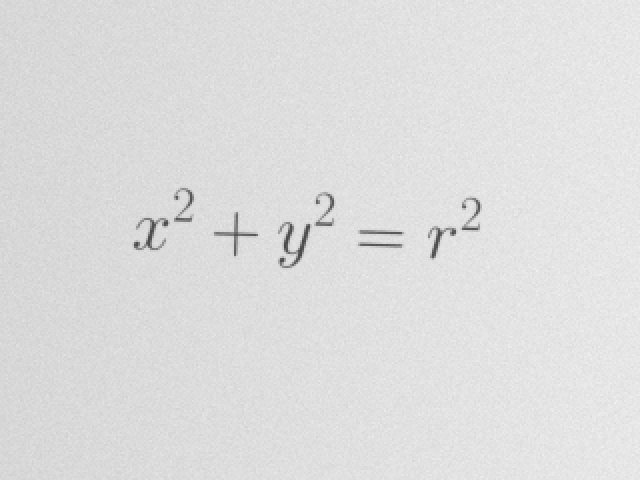
\includegraphics[width=0.47\linewidth]{img/fake_T26.png}\hfill
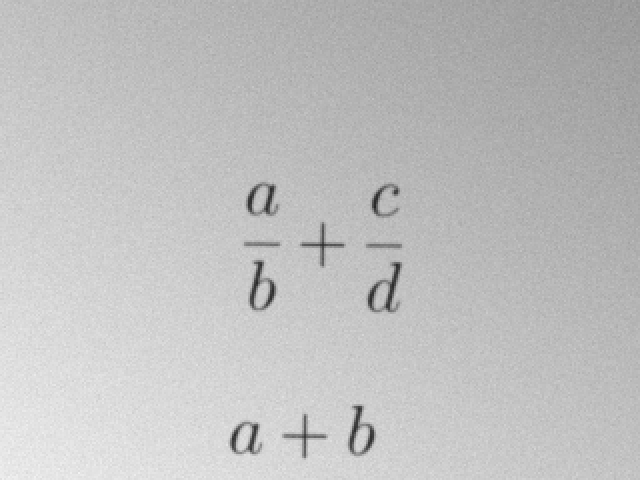
\includegraphics[width=0.47\linewidth]{img/fake_T47.png}
\caption{Two of the simulated photographs, \file{T26.png} and \file{T47.png}, shown enlarged.
A real frame from the board has the same size and a similar quality. Part of a neighbouring
printed line is visible at the bottom of the second photograph, as it would be on a real page;
the pipeline reads the line nearest the centre.}
\label{fig:fake}
\end{figure}

\begin{iffail}
If the output ends with \emph{pdflatex failed}, MiKTeX is not working: repeat
Steps~\ref{st:newafterinstall} to~\ref{st:verifytools}. If it says that \emph{pdftoppm (poppler)
is needed}, Poppler is not found: see Section~\ref{sec:trouble}. If a dialog of MiKTeX asks for
permission to install a package, click \ui{Install}, and afterwards run the command of
Step~\ref{st:autoinstall} again so that the question is not asked in future.
\end{iffail}

\subsection{Training images}

\step{Generate the synthetic training set}\label{st:synth}
\begin{ps}
python -m model.make_synthetic
\end{ps}
A classifier learns from examples. This command produces them without a camera: it draws every
one of the 182 symbols in every suitable font found on the laptop, and passes each drawing
through the same simulated camera as before, some 400 times per class with different sizes,
tilts, stroke weights and lighting.
\begin{out}[What you should see (abridged; the lead's laptop, 23 November)]
glyph bank: 6090 drawings from 31 font files + 5 mathtext sets; fewest: [...]; missing: []
bank built in 63 s -> C:\ee105\camera-to-latex\data\synthetic\glyph_bank.pkl
64600 crops for 159 classes in 20 s -> C:\ee105\camera-to-latex\data\synthetic\train.npz
segmentation check - members often split into pieces (tune MERGE_* in config.py):
  parallel         kept whole in 33% of drawings
  ...
preview pages: C:\ee105\camera-to-latex\data\synthetic/preview_*.png
\end{out}
\checkpoint{A line reports about 64{,}600 crops for 159 classes, and the list after
\emph{missing:} is empty (\texttt{[]}). The number of font files depends on the fonts installed
on the laptop and will differ from 31; that is expected. The lines about symbols ``split into
pieces'' are a diagnostic, not an error.}

To see what the classifier will learn from, run \code|explorer data\synthetic| and open
\file{preview\_1.png}: each row shows several generated images of one class.

\subsection{The classifier}

\step{Prepare the laptop for a long computation}
Training takes 45 to 75 minutes of uninterrupted computation. Connect the charger. Then make
sure that the laptop does not go to sleep: open \menu{Settings}\then\menu{System}\then\menu{Power
\& battery} (Windows~11) or \menu{Settings}\then\menu{System}\then\menu{Power \& sleep}
(Windows~10) and set the time after which the device sleeps \emph{when plugged in} to
\emph{Never}. Note the previous value so that you can restore it afterwards. Do not close the
lid during training.
\checkpoint{The charger is connected and sleep is switched off.}

\step{Train the convolutional neural network}\label{st:train}
\begin{ps}
python -m model.train
\end{ps}
The command reads the synthetic images, keeps 5\,\% of them aside for checking, and adjusts the
149{,}311 numerical weights of the network so that its answers on the remaining images improve.
One pass through all images is called an \term{epoch}; at most 30 are run, and training stops
earlier when the accuracy on the images kept aside has not improved for five epochs.
\begin{out}[What you should see at the start]
synthetic C:\ee105\camera-to-latex\data\synthetic\train.npz: 64600 crops
real crops: 0 (0 held out for testing)
training on 61385 crops, 159 classes, backend keras
model: 149311 weights
Epoch 1/30
\end{out}
After each epoch, which takes between one and three minutes, a line of figures is printed. The
figure to watch is \texttt{val\_accuracy}, the share of the images kept aside that were
classified correctly; it should rise above 0.9 within the first few epochs. Any lines about
\emph{oneDNN} or \emph{GPU support} at the start are informational. When training has finished,
a summary in braces is printed:
\begin{out}[What you should see at the end (the lead's laptop, 23 November)]
Epoch 24/30
480/480 - 86s - 179ms/step - accuracy: 0.9787 - loss: 0.0643 - val_accuracy: 0.9816 - val_loss: 0.0583 - learning_rate: 1.5625e-05
{
 "name": "symbols_v1",
 "backend": "keras",
 "crop_size": 32,
 "window_scale": 1.5,
 "features": "pixels",
 "weights": 149311,
 "trained": "2026-11-23 14:43",
 "minutes": 47.3,
 "data": {
  "synthetic": 61385,
  "real": 0,
  "real_repeat": 5,
  "external": 0
 },
 "synthetic_val_accuracy": 0.9835147744945568
}
\end{out}
\checkpoint{The summary shows \texttt{"backend": "keras"} and a value of
\texttt{synthetic\_val\_accuracy} of about 0.98 (between 0.97 and 0.99). The classifier has been
saved as \file{models\bs symbols\_v1.keras}, with its description in
\file{models\bs symbols\_v1.json}.}

\begin{note}[If time is short: the fallback classifier]
The command \code|python -m model.train --backend sklearn| trains a simpler classifier in two to
three minutes. It needs no TensorFlow and is slightly less accurate (0.974 against 0.984 on the
images kept aside). The rest of the quick start works with either. When both have been
trained, the pipeline uses the neural network.
\end{note}

\begin{iffail}[If the laptop slept, or the window was closed, during training]
Nothing is damaged. Open a new PowerShell window (Step~\ref{st:openps}) and give the three
commands below, one after the other. The training starts again from the beginning.
\end{iffail}
\begin{ps}[After an interruption, command 1 of 3]
cd C:\ee105\camera-to-latex
\end{ps}
\begin{ps}[After an interruption, command 2 of 3]
.\.venv\Scripts\Activate.ps1
\end{ps}
\begin{ps}[After an interruption, command 3 of 3]
python -m model.train
\end{ps}

\subsection{Accuracy of the complete pipeline}

\step{Evaluate on the 80 simulated photographs}\label{st:eval}
\begin{ps}
python -m tools.eval_pipeline --images test_set\synthetic --split all
\end{ps}
For each photograph the command runs the whole pipeline, compares the resulting \LaTeX{} with
the correct answer, and checks that the result compiles. It prints one line per photograph,
beginning with \texttt{ok} for a line read exactly right and with \texttt{-{}-} otherwise, and
then a summary table.
\begin{out}[What you should see (the lead's laptop, 23 November; most lines omitted)]
-- T01 plain     expected Hello World                  got Hello \textbackslash{}\textbackslash{}ror]d
ok T06 plain     expected a+b=c                        got a+b=c
ok T26 scripts   expected x^{2}+y^{2}=r^{2}            got x^{2}+y^{2}=r^{2}
ok T47 fractions expected \frac{a}{b}+\frac{c}{d}      got \frac{a}{b}+\frac{c}{d}

category   lines   exact     TER  compiles  s/line
plain         38   71.1%    9.8%    100.0%    0.54
scripts       23   60.9%   12.8%    100.0%    0.62
fractions     12   83.3%    7.2%    100.0%    0.37
mixed          7   57.1%   29.5%    100.0%    0.73
all           80   68.8%   12.0%    100.0%    0.55

per-line results: C:\ee105\camera-to-latex\results\eval_all_20261123_1450.csv
\end{out}

The columns of the table have the following meanings.
\begin{itemize}
\item \textbf{exact} is the share of lines whose \LaTeX{} equals the expected \LaTeX{} after both
  have been written in a standard form, so that differences of spacing, optional braces and
  synonyms such as \code|\le| and \code|\leq| do not count as errors.
\item \textbf{TER}, the token error rate, measures how wrong the lines are on average. A
  \term{token} is one unit of \LaTeX{}: a command such as \code|\alpha|, a brace, or a single
  character. With $d$ the smallest number of token insertions, deletions and substitutions that
  turn the output into the expected line (the edit distance), and $n$ the number of tokens of
  the expected line,
  \[
    \mathrm{TER} = \frac{d(\text{output},\ \text{expected})}{n} ,
  \]
  so that one wrong token in a line of 20 tokens gives 5\,\%.
\item \textbf{compiles} is the share of output lines that \cmd{pdflatex} accepts.
\item \textbf{s/line} is the computing time per photograph, in seconds, without the compile
  check.
\end{itemize}

\checkpoint{The table is printed, the row \emph{all} shows 80 lines, and the column
\emph{compiles} shows 100\,\%. Your percentages need not equal the ones above, because each
laptop trains a slightly different classifier; an overall \emph{exact} value between about 60\,\%
and 80\,\% is in the expected range at this size of lettering.}

\rationale{The value of about 69\,\% is the project's present state, not a fault of your
installation. Most errors arise when thin strokes break apart or neighbouring letters touch in
so small a picture; the companion document describes the measures taken against this.}

\step{Produce the review document}\label{st:review}
\begin{ps}
python -m tools.review_results
\end{ps}
\begin{out}
review: C:\ee105\camera-to-latex\results\review_all_20261124_1012.pdf
\end{out}
The command writes a PDF in which each test line occupies one row: the photograph with the
boxes that the pipeline drew, the expected line as typeset mathematics, and the line that the
pipeline produced, in orange when it is wrong (Figure~\ref{fig:review}). Open the folder with
\begin{ps}
explorer results
\end{ps}
and double-click the newest file whose name begins with \file{review\_}. The variant
\code|python -m tools.review_results --only-wrong| lists the misread lines only.
\checkpoint{The PDF opens and shows 80 rows of photographs with results.}

\begin{figure}[H]
\centering
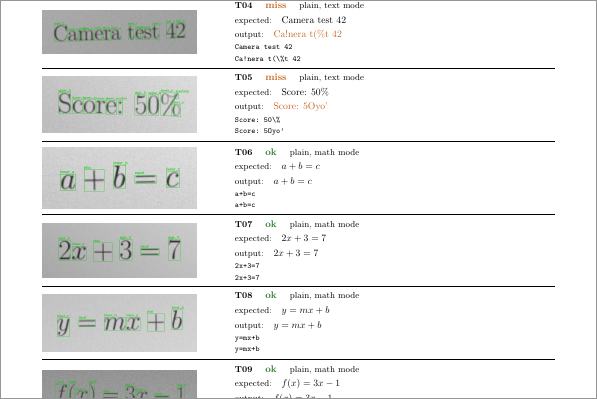
\includegraphics[width=0.86\linewidth]{img/review_page.png}
\caption{Part of a review document. Boxes in green mark symbols of which the classifier is
confident, boxes in red symbols of which it is not.}
\label{fig:review}
\end{figure}

\subsection{From one photograph to a PDF}

\step{Run the application on a stored photograph}\label{st:onephoto}
\begin{pswide}
python -m pipeline.main --new --image test_set\synthetic\T47.png --accept --pdf
\end{pswide}
This is the program that will later be used with the board, here given a stored photograph in
place of a live one. The option \code|--new| starts an empty document, \code|--accept| adds the
recognized line to it, and \code|--pdf| typesets the document and opens it.
\begin{out}
starting a new session
model symbols_v1 (keras, 159 classes)
test_set\synthetic\T47.png: [math] \frac{a}{b}+\frac{c}{d}  (612 ms)
accepted line 1: [math] \frac{a}{b}+\frac{c}{d}
PDF: C:\ee105\camera-to-latex\out\document.pdf
\end{out}
The time in parentheses will differ.
\checkpoint{A PDF opens in your PDF viewer and shows the sum of two fractions,
$\frac{a}{b}+\frac{c}{d}$, typeset as mathematics. If your classifier happened to misread a
symbol of this photograph the PDF shows that instead; the installation is correct either way,
because a PDF was produced.}

\subsection{Completion}

\step{Confirm the result and restore the power settings}
Tick the items of Table~\ref{tab:done}, restore the sleep setting that you changed before
training, and send the project lead a screenshot of the summary table of Step~\ref{st:eval}
(\key{Windows}+\key{Shift}+\key{S}).

\begin{table}[H]
\centering
\begin{tabular}{C{0.6cm}L{7.2cm}C{3.3cm}}
\toprule
 & \multicolumn{1}{c}{\hd{Result}} & \hd{Established in} \\
\midrule
\cbox & Four tools answer with a version number & Step~\ref{st:verifytools} \\
\cbox & The project is in \file{C:\bs ee105\bs camera-to-latex} & Step~\ref{st:gitclone} \\
\cbox & OpenCV 4 and TensorFlow 2 can be imported & Step~\ref{st:verifypy} \\
\cbox & All automatic tests pass & Step~\ref{st:pytest} \\
\cbox & 80 simulated photographs exist & Step~\ref{st:render} \\
\cbox & A classifier with about 98\,\% accuracy is stored in \file{models} & Step~\ref{st:train} \\
\cbox & The pipeline was scored on 80 lines, and every output compiled & Step~\ref{st:eval} \\
\cbox & One photograph became a PDF & Step~\ref{st:onephoto} \\
\bottomrule
\end{tabular}
\caption{Completion checklist for the set-up.}
\label{tab:done}
\end{table}

The quick start has created five folders inside the project: \file{data} (training images),
\file{models} (the classifier), \file{results} (evaluations), \file{out} (the PDF and its
sources) and \file{test\_set\bs synthetic} (the simulated photographs). Git is instructed, by
the file \file{.gitignore}, to leave all five on your laptop; they are never uploaded by
accident, and each can be regenerated with the commands of this section.

\section{Working routine}
\label{sec:routine}

The installation is done once. This section describes what is done every time: how a working
session begins, how results are shared with the team, and how a session ends.

\subsection{Begin a session}

\step{Open the project}
Open a new PowerShell window (Step~\ref{st:openps}) and give the opening sequence.
\begin{ps}[Opening sequence, command 1 of 2]
cd C:\ee105\camera-to-latex
\end{ps}
\begin{ps}[Opening sequence, command 2 of 2]
.\.venv\Scripts\Activate.ps1
\end{ps}
\checkpoint{The prompt reads:}
\venvprompt

\step{Fetch the team's latest changes}\label{st:pull}
\begin{ps}
git pull
\end{ps}
\begin{out}[What you should see when nothing has changed]
Already up to date.
\end{out}
When team members have uploaded changes since your last session, Git instead lists the files it
updated. Begin every session with this command; work done on an outdated copy is the usual
cause of the conflicts described below.
\checkpoint{The output is \emph{Already up to date} or a list of updated files, and it contains
neither \emph{error} nor \emph{CONFLICT}.}

\subsection{Share your work}

Sharing a change takes three commands: \cmd{git add} selects the files, \cmd{git commit} records
them on your laptop with a describing sentence, and \cmd{git push} uploads the record to GitHub.
The companion document gives these commands in full, with the real file names, at every point
where something is to be shared. Their general form is shown here.

\step{See what has changed}
\begin{ps}
git status
\end{ps}
\begin{out}[What you should see when you have changed the file config.py]
On branch main
Your branch is up to date with 'origin/main'.

Changes not staged for commit:
        modified:   config.py
\end{out}
\checkpoint{Every file listed is one that you meant to change. If a file is listed that you did
not mean to change, do not continue; ask the lead.}

\step{Select, record and upload}
In the first command, replace the placeholder by the name of the changed file as \cmd{git
status} printed it. In the second, replace the placeholder by a short sentence that says what
you did; keep the quotation marks.
\begin{center}
\texttt{git add }\ph{FILE}\\[4pt]
\texttt{git commit -m "}\ph{MESSAGE}\texttt{"}\\[4pt]
\texttt{git push}
\end{center}
\begin{out}[Example: sharing a change of config.py]
(.venv) PS C:\ee105\camera-to-latex> git add config.py
(.venv) PS C:\ee105\camera-to-latex> git commit -m "Set camera orientation"
[main 3f2c1ab] Set camera orientation
 1 file changed, 2 insertions(+), 2 deletions(-)
(.venv) PS C:\ee105\camera-to-latex> git push
To https://github.com/ashahvos/camera-to-latex.git
   a1b2c3d..3f2c1ab  main -> main
\end{out}
\checkpoint{The output of \cmd{git push} ends with a line of the form \texttt{main -> main}.
The change is now visible on the repository's page on GitHub.}

Three rules keep the shared repository in order.
\begin{enumerate}
\item Name the files you add. Do not use commands that add ``everything''; they sweep up files
  that were never meant to be shared.
\item Write messages that a team member will understand in a week: \emph{Add photos of test
  lines T01 to T60}, not \emph{update}.
\item Never share passwords, and never try to add the folders \file{.venv}, \file{data} or
  \file{out}; Git ignores them for good reason.
\end{enumerate}

\subsection{When Git objects}

\step{If the upload is rejected}
\begin{out}[The message]
 ! [rejected]        main -> main (fetch first)
error: failed to push some refs to 'https://github.com/ashahvos/camera-to-latex.git'
\end{out}
Someone uploaded a change after your last \cmd{git pull}. Nothing is lost. Fetch their change
and upload again:
\begin{ps}
git pull
\end{ps}
\begin{ps}
git push
\end{ps}
If Notepad opens during \cmd{git pull} with a sentence that begins \emph{Merge branch}, Git is
proposing a description for the combination of the two changes. The proposal is adequate: close
Notepad (\menu{File}\then\menu{Exit}), and the command completes.

\step{If Git reports a conflict}
\begin{out}[The message]
CONFLICT (content): Merge conflict in config.py
Automatic merge failed; fix conflicts and then commit the result.
\end{out}
You and a team member changed the same lines of the same file, and Git cannot decide between
the two versions. Return the project to its state before the pull with
\begin{ps}
git merge --abort
\end{ps}
and send the lead a screenshot. Your own change is still recorded on your laptop; the lead will
say which version should prevail.
\checkpoint{\cmd{git status} no longer mentions a merge.}

\step{If Git refuses to pull because of local changes}
\begin{out}[The message]
error: Your local changes to the following files would be overwritten by merge:
\end{out}
You changed a file without recording the change, and the same file has changed on GitHub.
Record your change first (the \cmd{git add} and \cmd{git commit} commands above), then run
\cmd{git pull} again.

\subsection{End a session}

\step{Close the window}
When the prompt is showing, type \code|exit| and press \key{Enter}, or close the window with
the \ui{X} button. Nothing needs to be saved or switched off; the environment is simply
activated again by the opening sequence next time.

\begin{caution}[Do not update the software before the hand-in]
The versions installed by this guide are known to work together. Until the project has been
handed in on December~1, decline offers to upgrade Python packages (including the notice that a
new version of pip is available), and do not run commands that upgrade them. A working
installation is worth more than a current one.
\end{caution}

\section{Troubleshooting}
\label{sec:trouble}

The entries below are ordered by the stage at which the message appears. Each quotes the
characteristic part of the message, in the form in which PowerShell prints it. Red text is
PowerShell's way of marking an error; read its first line, which names the cause, and ignore
the lines beginning with a plus sign that follow it.

Several remedies ask for the \emph{opening sequence}. It consists of the following two
commands, given in this order in a PowerShell window; afterwards the prompt begins with
\texttt{(.venv)}.
\begin{ps}[Opening sequence, command 1 of 2]
cd C:\ee105\camera-to-latex
\end{ps}
\begin{ps}[Opening sequence, command 2 of 2]
.\.venv\Scripts\Activate.ps1
\end{ps}

\subsection{PowerShell and the tools}

\trouble{\texttt{brew : The term 'brew' is not recognized as the name of a cmdlet}}
\cause \cmd{brew} is the package manager of macOS. Instructions found on the internet often assume a
Mac.
\remedy Use only the commands of this guide; on Windows the corresponding program is \cmd{winget}.

\trouble{\texttt{winget : The term 'winget' is not recognized}}
\cause The Windows component \emph{App Installer} is missing or out of date.
\remedy Open Microsoft Store, search for \emph{App Installer}, click \ui{Get} or \ui{Update}, and
open a new PowerShell window.

\trouble{\texttt{git} (or \texttt{py}, \texttt{pdflatex}, \texttt{pdftoppm}) \texttt{: The
term \ldots{} is not recognized}}
\cause Either the window was opened before the program was installed, or the installation failed.
\remedy Open a new PowerShell window and try again. If the message persists, repeat the installation
step of that program in Section~\ref{sec:tools} and read its output for an error.

\trouble{\texttt{pdftoppm} is still not recognized after Poppler has been installed again}
\cause The folder that contains \file{pdftoppm.exe} is not on the list of folders that Windows
searches (the \term{path}).
\remedy Run the five commands below in order. The third must print the name of a folder that ends in
\file{Library\bs bin}; if it prints nothing, Poppler is not installed, and the remedy is to
repeat its installation step. After the fifth command, open a new PowerShell window and run
\texttt{pdftoppm -v}.
\begin{ps}[Repair of the search path, command 1 of 5]
cd "$env:LOCALAPPDATA\Microsoft\WinGet\Packages"
\end{ps}
\begin{ps}[Repair of the search path, command 2 of 5]
$p = Get-ChildItem -Recurse -Filter pdftoppm.exe
\end{ps}
\begin{ps}[Repair of the search path, command 3 of 5]
$p[0].DirectoryName
\end{ps}
\begin{ps}[Repair of the search path, command 4 of 5]
$old = [Environment]::GetEnvironmentVariable("Path", "User")
\end{ps}
\begin{pswide}[Repair of the search path, command 5 of 5]
[Environment]::SetEnvironmentVariable("Path", "$old;$($p[0].DirectoryName)", "User")
\end{pswide}

\trouble{\texttt{Python was not found; run without arguments to install from the Microsoft
Store}, or the Microsoft Store opens when a command beginning with \texttt{python} is run}
\cause The environment is not activated in this window, so Windows offers its own placeholder for
Python.
\remedy Check the prompt. If it does not begin with \texttt{(.venv)}, give the opening sequence
(the two commands at the head of this section).

\trouble{\texttt{py : The term 'py' is not recognized}, or \texttt{Python 3.12 not found}}
\cause Python 3.12 is not installed, or the window is older than the installation.
\remedy Open a new window. If the message persists, repeat the Python installation step of
Section~\ref{sec:tools}.

\trouble{\texttt{Activate.ps1 cannot be loaded because running scripts is disabled on this
system}}
\cause PowerShell's execution policy forbids scripts.
\remedy Run Step~\ref{st:policy} and answer \texttt{Y}. If the policy cannot be changed because the
laptop is managed by an organization, the environment can be used without activation: in every
command of this guide and its companion, write \code|.\.venv\Scripts\python.exe| in place of the
word \texttt{python} at the beginning, and \code|.\.venv\Scripts\python.exe -m pip| in place of
\texttt{pip}.

\trouble{\texttt{The module '.venv' could not be loaded}, with the activation line shown
twice in a row}
\cause The activation command was pasted twice before \key{Enter} was pressed.
\remedy Press \key{Esc} to clear the line, then paste the command once.

\trouble{\texttt{.\bs .venv\bs Scripts\bs Activate.ps1 : The term \ldots{} is not recognized}}
\cause The current folder is not the project folder, so there is no \file{.venv} in it.
\remedy Run \code|cd C:\ee105\camera-to-latex| first: the opening sequence has two commands, and the
order matters.

\trouble{\texttt{The '<' operator is reserved for future use}}
\cause A command copied from another source contained a placeholder in angle brackets, such as
\texttt{<your-username>}, and it was pasted without being replaced.
\remedy Use the commands of this guide, which contain no such placeholders.

\trouble{The window shows no new output and does not react}
\cause If the title bar contains the word \emph{Select}, a mouse click has paused the program.
Otherwise the command is probably still working.
\remedy Press \key{Esc} in the first case. In the second, wait; Steps~\ref{st:pipinstall}
and~\ref{st:train} state how long the slow commands may take.

\subsection{Python packages}

\trouble{\texttt{ERROR: Could not find a version that satisfies the requirement tensorflow}}
\cause The environment was created with a Python version for which TensorFlow is not published.
\remedy Run \code|python --version| with the environment activated. If it does not print
\texttt{Python 3.12}, close the window, delete the folder \file{.venv} in File Explorer, and
repeat Section~\ref{sec:python} from its second step, typing \texttt{py -3.12} exactly.

\trouble{\texttt{OSError: [Errno 2] No such file or directory} with the hint \texttt{Windows
Long Path support}}
\cause The project folder lies so deep in the folder tree that some file names of TensorFlow exceed
260 characters.
\remedy Install the project in \file{C:\bs ee105} as described in Section~\ref{sec:clone}, not in a
folder inside \file{Desktop} or \file{Documents}.

\trouble{\texttt{ReadTimeoutError}, or \texttt{Connection \ldots{} timed out}, during
\texttt{pip install}}
\cause The internet connection was interrupted.
\remedy Run the same command again. Packages already downloaded are not fetched a second time.

\trouble{\texttt{AttributeError: module 'cv2' has no attribute 'HOGDescriptor'}}
\cause Version~5 of OpenCV is installed.
\remedy Run Step~\ref{st:opencv}.

\trouble{\texttt{ModuleNotFoundError: No module named 'cv2'} (or \texttt{numpy},
\texttt{tensorflow})}
\cause The environment is not activated, or Step~\ref{st:pipinstall} did not finish.
\remedy Check for \texttt{(.venv)} in the prompt; if it is present, run Step~\ref{st:pipinstall}
again.

\trouble{\texttt{No module named pipeline} (or \texttt{tools}, \texttt{model})}
\cause The command was run outside the project folder.
\remedy Run \code|cd C:\ee105\camera-to-latex| and repeat the command.

\trouble{\texttt{ImportError: DLL load failed while importing \_pywrap\_tensorflow\_internal}}
\cause A Microsoft runtime library that TensorFlow requires is missing from Windows.
\remedy Run \code|winget install --id Microsoft.VCRedist.2015+.x64 -e --source winget|, open a new
window, give the opening sequence (the two commands at the head of this section), and repeat
Step~\ref{st:verifypy}.

\trouble{Lines that mention \texttt{oneDNN custom operations}, \texttt{absl::InitializeLog}
or \texttt{GPU support is not available on native Windows}}
\cause TensorFlow announces how it will compute. On Windows it uses the processor, not a graphics
card, which is sufficient for this project.
\remedy None is needed; these are not errors.

\subsection{\LaTeX{} and Poppler}

\trouble{\texttt{'pdflatex' is not on PATH}, or \texttt{'pdflatex' not found}}
\cause MiKTeX is not installed, or the window is older than its installation.
\remedy Open a new window. If the message persists, repeat the MiKTeX steps of
Section~\ref{sec:tools}.

\trouble{\texttt{pdflatex took longer than 20 s}}
\cause MiKTeX was downloading a component, or was waiting behind a dialog for permission to do so.
\remedy Look for a MiKTeX dialog behind the other windows and click \ui{Install}. Run
Step~\ref{st:autoinstall}, then repeat the command; the second attempt is fast because the
component is now present.

\trouble{\texttt{pdflatex failed:} followed by \texttt{LaTeX Error: File \ldots{} not found}}
\cause MiKTeX could not fetch a component, usually because it has never synchronized with its
servers or because there is no internet connection.
\remedy Open MiKTeX Console, click \ui{Check for updates}, install what is offered, and repeat the
command.

\trouble{\texttt{RuntimeError: pdftoppm (poppler) is needed for -{}-render}}
\cause Poppler is not installed or not found.
\remedy Run \texttt{pdftoppm -v} in a new window and follow the first entries of this section.

\subsection{Commands of the project}

\trouble{\texttt{symbols\_v1.json not found: train a model first}}
\cause No classifier has been trained on this laptop yet.
\remedy Run Steps~\ref{st:synth} and~\ref{st:train}.

\trouble{\texttt{missing \ldots{}train.npz: run python -m model.make\_synthetic first}}
\cause Training was started before the training images were generated.
\remedy Run Step~\ref{st:synth}, then Step~\ref{st:train}.

\trouble{\texttt{no photos found in test\_set\bs images for split test}}
\cause The evaluation was run without its two options, so it looked for photographs taken with the
board, which do not exist yet.
\remedy Use the full command of Step~\ref{st:eval}, which ends in
\code|--images test_set\synthetic --split all|.

\trouble{\texttt{no results file: run python -m tools.eval\_pipeline first}}
\cause The review document is built from an evaluation, and none has been run.
\remedy Run Step~\ref{st:eval}, then Step~\ref{st:review}.

\trouble{\texttt{camera problem:} followed by a remark about ports}
\cause The application was started without the option \texttt{-{}-image} and looked for the board.
\remedy Use the full command of Step~\ref{st:onephoto}. Work with the board is described in the
companion document.

\subsection{Git}

\trouble{\texttt{remote: Repository not found.}}
\cause Your GitHub account has no access to the repository, or the wrong account is signed in.
\remedy See the amber box of Step~\ref{st:gitclone}.

\trouble{\texttt{fatal: destination path 'camera-to-latex' already exists and is not an
empty directory}}
\cause The repository was cloned earlier.
\remedy Nothing; continue with the step after the clone.

\trouble{\texttt{Author identity unknown} \ldots{} \texttt{Please tell me who you are}}
\cause Git does not know your name and email address.
\remedy Carry out the subsection \emph{Introduce yourself to Git} of Section~\ref{sec:clone}.

\trouble{\texttt{fatal: not a git repository}}
\cause The current folder is not the project folder.
\remedy Run \code|cd C:\ee105\camera-to-latex|.

\trouble{\texttt{[rejected] main -> main}, \texttt{CONFLICT}, or \texttt{Your local changes
\ldots{} would be overwritten}}
\cause The team's copy and yours have diverged.
\remedy Section~\ref{sec:routine} treats each of the three cases.

\subsection{The laptop}

\trouble{An installation inside \file{Desktop} or \file{Documents} is extremely slow}
\cause OneDrive synchronizes those folders and uploads every file of the environment.
\remedy Keep the project in \file{C:\bs ee105}. If it was cloned elsewhere, delete that copy and
repeat Sections~\ref{sec:clone} and~\ref{sec:python}.

\trouble{Training stopped because the laptop went to sleep}
\cause The power settings suspended the computation.
\remedy Switch sleep off while the charger is connected, as described before Step~\ref{st:train}, and
start the training again.

\appendix
\section{Glossary}
\label{sec:glossary}

\begin{description}[style=nextline,leftmargin=1.6em,itemsep=3pt]
\item[Activation] The act of telling one PowerShell window to use the project's virtual
  environment. Shown by \texttt{(.venv)} at the start of the prompt.
\item[Board] The USC EE\,105 circuit board with its Arduino Nano 33 BLE Sense Lite and OV7675
  camera. In this project it only takes photographs.
\item[Classifier] The part of the pipeline that names a symbol from its picture. The project's
  classifier is a convolutional neural network.
\item[Clone] A complete copy of a repository on your own computer, or the act of making one.
\item[CNN (convolutional neural network)] A neural network designed for images. It applies
  small filters across the picture to detect strokes and corners and combines their responses
  into a decision.
\item[Commit] A recorded state of the repository, with an author, a date and a message; also the
  act of recording one.
\item[Current folder] The folder in which PowerShell carries out a command, shown in the prompt.
\item[Epoch] One pass of the training procedure through all training images.
\item[Frame] One photograph from the camera: $320 \times 240$ pixels, each a gray level from 0
  (black) to 255 (white).
\item[Git] The program that records and exchanges the history of a repository.
\item[GitHub] The website on which the team's repository is stored.
\item[\LaTeX{}] A typesetting system in which a document is written as text with commands, for
  example \code|\frac{a}{b}| for a fraction, and converted to a PDF by a program such as
  \cmd{pdflatex}.
\item[MiKTeX] The distribution of \LaTeX{} for Windows used here.
\item[Package] A unit of software written by others and installed by a package manager:
  \cmd{pip} for Python packages, \cmd{winget} for Windows programs, MiKTeX for \LaTeX{}
  components.
\item[Path] In the narrow sense, the location of a file, such as
  \code|C:\ee105\camera-to-latex\config.py|. In the phrase ``on the path'', the list of folders
  in which Windows looks for a program whose name is typed.
\item[Pipeline] The chain of processing stages from photograph to PDF
  (Figure~\ref{fig:pipeline}).
\item[Prompt] The text that PowerShell prints when it is ready for a command.
\item[Pull, push] To fetch the team's commits from GitHub, and to upload one's own.
\item[Repository] A folder whose history is managed by Git.
\item[Segmentation] The stage that finds the individual symbols in a photograph.
\item[Token] One unit of \LaTeX{} text: a command, a brace or a single character.
\item[Virtual environment] A private installation of Python and its packages inside the
  project folder \file{.venv}.
\end{description}

\section{Summary of commands}
\label{sec:summary}

Table~\ref{tab:cmds} lists the commands of the guide for later reference. All but the first
group are run in the project folder with the environment activated.

\begin{table}[H]
\footnotesize
\noindent\hspace*{-12mm}%
\begin{tabular}{L{11.0cm}L{3.3cm}}
\toprule
\multicolumn{1}{c}{\hd{Command}} & \multicolumn{1}{c}{\hd{Effect}} \\
\midrule
\multicolumn{2}{l}{\emph{Opening sequence, in every new PowerShell window}} \\
\lstinline[style=sum]|cd C:\ee105\camera-to-latex| & Go to the project \\
\lstinline[style=sum]|.\.venv\Scripts\Activate.ps1| & Activate environment \\
\midrule
\multicolumn{2}{l}{\emph{Project}} \\
\lstinline[style=sum]|python -m pytest -q| & Run the automatic tests \\
\lstinline[style=sum]|python -m tools.make_test_lines --render| & Simulated photographs \\
\lstinline[style=sum]|python -m model.make_synthetic| & Training images \\
\lstinline[style=sum]|python -m model.train| & Train the classifier \\
\lstinline[style=sum]|python -m tools.eval_pipeline --images test_set\synthetic --split all| & Score the pipeline \\
\lstinline[style=sum]|python -m tools.review_results| & Review document \\
\lstinline[style=sum]|python -m pipeline.main --image test_set\synthetic\T47.png --accept --pdf| & One photograph to PDF \\
\midrule
\multicolumn{2}{l}{\emph{Git}} \\
\lstinline[style=sum]|git pull| & Fetch team's changes \\
\lstinline[style=sum]|git status| & List changed files \\
\lstinline[style=sum]|git add|, \lstinline[style=sum]|git commit -m|, \lstinline[style=sum]|git push| & Select, record, upload \\
\midrule
\multicolumn{2}{l}{\emph{PowerShell}} \\
\lstinline[style=sum]|cls| & Clear the window \\
\lstinline[style=sum]|explorer .| & Open the current folder \\
\lstinline[style=sum]|exit| & Close the window \\
\bottomrule
\end{tabular}
\normalsize
\caption{The commands used in this guide. Each command is one line.}
\label{tab:cmds}
\end{table}

\section{Removing the installation}

Nothing in this guide alters Windows irreversibly. To remove the project from a laptop, delete
the folder \file{C:\bs ee105} in File Explorer; this removes the code, the environment and all
generated data. To remove the tools, open \menu{Settings}\then\menu{Apps}\then\menu{Installed
apps} and uninstall \emph{Git}, \emph{Python 3.12}, \emph{Python Launcher}, and \emph{MiKTeX}.
Poppler is removed with the command
\code|winget uninstall --id oschwartz10612.Poppler|. The GitHub account is independent of the
laptop and remains.

\section{Sources}

The installation procedure follows the publishers' own instructions, consulted on 24 November
2026.
\begin{itemize}
\item GitHub Docs, \emph{Creating an account on GitHub}:
  \url{https://docs.github.com/en/get-started/start-your-journey/creating-an-account-on-github}
\item GitHub Docs, \emph{Inviting collaborators to a personal repository}:
  \url{https://docs.github.com/en/repositories/managing-your-repositorys-settings-and-features/repository-access-and-collaboration/inviting-collaborators-to-a-personal-repository}
\item GitHub Docs, \emph{Caching your GitHub credentials in Git} (Git Credential Manager):
  \url{https://docs.github.com/en/get-started/git-basics/caching-your-github-credentials-in-git}
\item Microsoft Learn, \emph{Use the WinGet tool to install and manage applications}:
  \url{https://learn.microsoft.com/en-us/windows/package-manager/winget}
\item Python documentation, \emph{Using Python on Windows} (version 3.12):
  \url{https://docs.python.org/3.12/using/windows.html}
\item MiKTeX, \emph{Install MiKTeX on Windows}: \url{https://miktex.org/howto/install-miktex}
\item MiKTeX, \emph{Just enough TeX} (automatic installation of packages):
  \url{https://miktex.org/kb/just-enough-tex}
\item Poppler packaged for Windows: \url{https://github.com/oschwartz10612/poppler-windows}
\end{itemize}
The expected outputs of the project's own commands were taken from runs of the repository on the
project lead's Windows laptop on 23 November 2026, and from runs of the same commands in a Linux
test environment on 24 November 2026.

\end{document}
